%
%  $Author: ienne $
%  $Date: 1995/09/15 15:20:59 $
%  $Revision: 1.4 $
%

% \documentclass[10pt,journal,cspaper,compsoc]{IEEEtran}   %%%tc version
\documentclass[10pt, conference]{IEEEtran}
%\documentclass[conference,compsoc]{IEEEtran}
%\documentclass[10pt, conference]{IEEEtran}
%\documentclass[times, 10pt,onecolumn]{article}
\usepackage{amsmath, amssymb, enumerate}
\usepackage{semantic}
\usepackage{soul}
\usepackage{listings}

%%%%%%%%%%%%%%%% page control%%%%%%%%%%%%%%%%%
%\usepackage[margin=0.75in]{geometry}

%\linespread{0.991}  %%%%%%%%%%%%%%%%%%%%%%%%%%%%%%%%% this is really useful
%\usepackage{cite}
\usepackage{fancybox}
\usepackage{amsfonts}
%\usepackage{algorithm}
%\usepackage[noend]{algorithmic}
\usepackage[usenames]{color}
%\usepackage{colortbl}
%\usepackage[ figure, boxed, vlined]{algorithm2e}
%\usepackage[linesnumbered,vlined]{algorithm2e}
%\usepackage[lined,boxed]{algorithm2e}
\usepackage{listings}

\usepackage[linesnumbered,vlined]{algorithm2e}
\usepackage{graphicx}
\usepackage{times}
\usepackage{psfrag}
\usepackage{subfigure}
\usepackage{caption}
%\usepackage{subcaption}
\usepackage{multirow}
%\usepackage{setspace}
%\usepackage{listings}
\usepackage{epsfig}
%\usepackage{epstopdf}
%\usepackage[font=small,labelfont=bf]{caption}
% \usepackage{url}
\usepackage[hyphens]{url}

\usepackage{color}
\def\fixme#1{\typeout{FIXED in page \thepage : {#1}}
%\bgroup \color{red}{} \egroup}
\bgroup \color{red}{[FIXME: {#1}]} \egroup}

\lstset{breaklines=true, basicstyle=\ttfamily\fontsize{6}{7}\selectfont, escapeinside={(*@}{@*)}}

%\usepackage[pdftex]{hyperref}
\usepackage{rotating,tabularx}

\interfootnotelinepenalty=10000

%% Define a new 'leo' style for the package that will use a smaller font.
\makeatletter
\def\url@leostyle{%
  \@ifundefined{selectfont}{\def\UrlFont{\sf}}{\def\UrlFont{\small\ttfamily}}}
\makeatother

%\documentstyle[times,art10,twocolumn,latex8]{article}

%-------------------------------------------------------------------------
% take the % away on next line to produce the final camera-ready version
\pagestyle{plain}
%\thispagestyle{empty}
%\pagestyle{empty}

\newtheorem{theorem}{Theorem}
\newtheorem{lemma}[theorem]{Lemma}


%% remaining budget share, used in task stall section.
\newcommand{\bottomrule}{\hline}
\newcommand{\toprule}{\hline}
\newcommand{\midrule}{\hline}

\setlength\extrarowheight{1.5pt}
\setlength{\tabcolsep}{1pt}

\newcommand{\ttt}{\texttt}
\newcommand{\rarr}{\rightarrow}
\newcommand{\sarr}{\leadsto}

% \addtolength{\jot}{3mm}

%-------------------------------------------------------------------------
\begin{document}

\title{A Domain Specific Language for SpectreGuard}
\author{David Young\\
d063y800@ku.edu\\
University of Kansas, USA\\
}

\maketitle
\thispagestyle{empty}
\begin{abstract}

  A Spectre mitigation strategy in the form of a mechanism for marking variables
  as "non-speculative" was developed in \cite{SpectreGuard}. In this paper, we
  develop an embedded domain specific language (EDSL) in Haskell to provide
  support for this feature, with a backend that generates C code. The static
  type system of Haskell is used so that many basic forms of copying secret
  variables to public variables are disallowed. Additionally, a static analysis
  was developed which will detect some cases of secret variables leaking to
  public variables via control flow constructs.

\end{abstract}

%-------------------------------------------------------------------------

\section{Introduction}
Introduction goes here.

\section{Background}
Cite a paper. % \cite{barroso2009datacenter}.

Cite multiple papers. % \cite{banga99resourcecontainers,barroso2009datacenter}

\section{Syntax}
A correspondence between the syntax of the EDSL, which is inherited from
Haskell, and the C language is given in Fig. \ref{fig:Syntax}. In the right column, an
overline indicates that the transformation from EDSL to C is recursively
performed to the expression or command underneath the overline.

This also outlines procedure that the C code generator uses.

\begin{figure}[h]
\begin{tabular}{|l|l|}
  \hline
  EDSL syntax & C syntax \\
  \hline
  \begin{lstlisting}
  v <- decl x
  \end{lstlisting}
  & \begin{lstlisting}[language=C]
  int v = x;
  \end{lstlisting}\\

  \hline
  \begin{lstlisting}
  v <- allocPublic @Int n
  \end{lstlisting}
  & \begin{lstlisting}[language=C]
  int v[n];
  \end{lstlisting}\\

  \hline
  \begin{lstlisting}
  v <- allocPrivate @Int n
  \end{lstlisting}
  & \begin{lstlisting}[language=C]
  int v[n] __attribute__((__nospec__));
  \end{lstlisting}\\

  \hline
  \begin{lstlisting}
  arrA .= arrB
  \end{lstlisting}
  & \begin{lstlisting}[language=C]
  memcpy(arrA, arrB, sizeof(arrA));
  \end{lstlisting}\\

  \hline
  \begin{lstlisting}
  i .= j
  \end{lstlisting}
  & \begin{lstlisting}[language=C]
  i = j;
  \end{lstlisting}\\

  \hline
  \begin{lstlisting}
  arr ! i
  \end{lstlisting}
  & \begin{lstlisting}[language=C]
  arr[i]
  \end{lstlisting}\\

  \hline
  \begin{lstlisting}
  x <? y
  \end{lstlisting}
  & \begin{lstlisting}[language=C]
  x < y
  \end{lstlisting}\\

  \hline
  \begin{lstlisting}
  while cond body
  \end{lstlisting}
  & \begin{lstlisting}[language=C]
  while ((*@$\overline{\ttt{cond}}$@*)) { (*@$\overline{\ttt{body}}$@*) }
  \end{lstlisting}\\

  \hline
  \begin{lstlisting}
  ifThenElse cond t f
  \end{lstlisting}
  & \begin{lstlisting}[language=C]
  if ((*@$\overline{\ttt{cond}}$@*)) { (*@$\overline{\ttt{t}}$@*) } else { (*@$\overline{\ttt{f}}$@*) }
  \end{lstlisting}\\

  \hline
  \begin{lstlisting}
  for init
    (\i ->
      (cond, update, body))
  \end{lstlisting}
  & \begin{lstlisting}[language=C]
  for (int i = (*@$\overline{\ttt{init}}$@*); (*@$\overline{\ttt{cond}}$@*); (*@$\overline{\ttt{update}}$@*))
    { (*@$\overline{\ttt{body}}$@*) }
  \end{lstlisting}\\


  \hline
\end{tabular}
\caption{Syntax of the EDSL vs C syntax}
\label{fig:Syntax}
\end{figure}

\section{Sensitivity Types}
The Haskell type system is leveraged to perform a basic static consistency check of the sensitivities
of variables, so that a variable does not get assigned to a variable of a different sensitivity. This
is done by making the \verb|Expr| type constructor take a phantom type argument~\cite{Phantom}. The
logical inference rules corresponding to this check are given in Fig. \ref{fig:SensTypes}. An introduction
to this style of inference rule system, with many examples and applications in the study of programming languages, is given in \cite{HarperFoundations}.

Singletons~\cite{SingletonsPaper} are used to preserve this type level at runtime, so that the
code generator can generate SpectreGuard annotations where appropriate.

In Fig. \ref{fig:SensTypes}, it is assumed that $\tau$ and $\sigma$ are given by the
following grammar:
\begin{gather*}
  \sigma ::= \ttt{Public}\;|\;\ttt{Secret}\\
  \tau ::= \ttt{Int}\;|\;\ttt{Ptr}\;\tau\\
  \alpha ::= \ttt{Cmd ()}\;|\;\ttt{Cmd (Expr $\sigma$ $\tau$)}
\end{gather*}

A typing judgement is expressed with the syntax

\begin{equation*}
  \ttt{x :: $\beta$}
\end{equation*}

where \ttt{x} is some expression or command in the EDSL. This judgement means
that \ttt{x} has type $\beta$. This is also the same syntax used by Haskell, and by extension
the EDSL, to explicitly specify the type of any expression when necessary or desired.


\begin{figure}[h]
  \centering
\resizebox{0.68\linewidth}{!}{
\begin{minipage}{\linewidth}
  \centering
  \openup 3mm
\begin{gather*}
  \inference{}{\ttt{Public :: Sensitivity}}\\
  \inference{}{\ttt{Secret :: Sensitivity}}\\
  \inference{n \in \mathbb{N}}{\ttt{$n$ :: Int}}\\
  \inference{n \in \mathbb{N}}{\ttt{$n$ :: Expr $\sigma$ Int}}\\
  \inference{%
    \Gamma \vdash \ttt{x :: Expr $\sigma$ Int}
    & \Gamma \vdash \ttt{y :: Expr $\sigma$ Int}}
    {\Gamma \vdash \ttt{x + y :: Expr $\sigma$ Int}}\\
  \inference{%
    \Gamma \vdash \ttt{x :: Expr $\sigma$ Int}
    & \Gamma \vdash \ttt{y :: Expr $\sigma$ Int}}
    {\Gamma \vdash \ttt{x <? y :: Expr $\sigma$ Bool}}\\
  \inference{%
    \Gamma \vdash \ttt{a :: Expr $\sigma$ (Ptr $\tau$)}
    & \Gamma \vdash \ttt{i :: Expr $\sigma$ Int}}
    {\Gamma \vdash \ttt{a ! i :: Expr $\sigma$ $\tau$}}\\
  \inference{\Gamma \vdash \ttt{n :: Int}}{\Gamma \vdash \ttt{allocPublic @$\tau$ n :: Cmd (Expr Public (Ptr $\tau$))}}\\
  \inference{\Gamma \vdash \ttt{n :: Int}}{\Gamma \vdash \ttt{allocSecret @$\tau$ n :: Cmd (Expr Secret (Ptr $\tau$))}}\\
  \inference{\Gamma \vdash \ttt{x :: $\tau$}}{\Gamma \vdash \ttt{decl x :: Cmd (Expr Public $\tau$)}}\\
  \inference{%
    \Gamma \vdash \ttt{x :: Expr $\sigma$ $\tau$}
    & \Gamma \vdash \ttt{y :: Expr $\sigma$ $\tau$}}
    {\Gamma \vdash \ttt{x .= y :: Cmd ()}}\\
  \inference{%
    \Gamma \vdash \ttt{cond :: Expr $\sigma$ Bool}
    &\Gamma \vdash \ttt{t :: $\tau$}
    &\Gamma \vdash \ttt{f :: $\tau$}}
    {\Gamma \vdash \ttt{ifThenElse cond t f :: Cmd ()}}\\
  \inference{%
    \Gamma \vdash \ttt{cond :: Expr $\sigma$ Bool}
    & \Gamma \vdash \ttt{body :: Cmd $\alpha$}}
    {\Gamma \vdash \ttt{while cond body :: Cmd ()}}\\
  \inference{%
    \Gamma \vdash \ttt{init :: Expr $\sigma$ $\tau$}\\
    \Gamma \vdash \ttt{fn :: Expr $\sigma$ $\tau$ $\rarr$ (Expr $\sigma$ Bool, Cmd (), Cmd ())}
    }{\Gamma \vdash \ttt{for init fn :: Cmd ()}}\\
  \inference{%
    \Gamma \vdash \ttt{c :: Cmd (Expr $\sigma$ $\tau$)}
    & \ttt{x} \notin dom(\Gamma)
    \\ \Gamma \vdash \ttt{($\lambda$ x $\rarr$ body) :: Expr $\sigma$ $\tau$ $\rarr$ Cmd $\alpha$}
  }{%
    \Gamma \vdash \ttt{(\textbf{do} \{ x <- c; body \}) :: Cmd $\alpha$}
  }
\end{gather*}
\end{minipage}}
  \caption{Typing rules for sensitivity types}
\label{fig:SensTypes}
\end{figure}

...

\section{Examples}
\label{sec:Examples}

A couple of simple examples illustrate the basic typing rules:

\begin{lstlisting}[language=haskell]
example1 :: Cmd ()
example1 = do
  array1 <- allocSecret @Int 8
  array2 <- allocSecret @Int 8
  array2 .= array1
\end{lstlisting}

\noindent This first example passes the type checker with no problem: the array copy
is being performed from one secret array to another secret array.

The next example does not type check:

\begin{lstlisting}[language=haskell]
  -- This example fails to type check
example2 :: Cmd ()
example2 = do
  array1 <- allocSecret @Int 8
  array2 <- allocPublic @Int 8
  (*@\color{red}array2 .= array1@*)
\end{lstlisting}

\noindent \ttt{example2} fails to type check since \ttt{array1} and \ttt{array2} have
different sensitivity annotations, while the type of the \ttt{(.=)} operation
requires that both arguments have the same sensitivity annotation. This restriction can
be seen in the typing rule for \ttt{(.=)} in Fig. \ref{fig:SensTypes}.

Turning to more complex examples, we can see that the following example type checks

\begin{lstlisting}[language=Haskell]
example3 :: Cmd ()
example3 = do
  arrayA <- allocSecret @Int 8
  arrayB <- allocSecret @Int 8
  for (0 :: Expr Secret Int) (\i -> ((i <? 8), (i += 1), do
    (arrayA ! i) .= (arrayB ! i)))
\end{lstlisting}

\noindent This demonstrates a basic \ttt{for} loop and the array indexing syntax. Again, the
only copies happen between two variables with the same sensitivity level, so this
program is well-typed.

The next slightly more complex example exhibits an important limitation of this sensitivity type checking:

\begin{lstlisting}[language=Haskell]
example4 :: Cmd ()
example4 = do
  secretArray <- allocSecret @Int 8
  publicArray <- allocPublic @Int 8

  for (0 :: Expr Public Int) (\i -> ((i <? 8), (i += 1), do
    leak <- decl (0 :: Int)
    for (0 :: Expr Secret Int) (\j -> ((j <? (secretArray ! i))
                                      ,(j += 1), do
      leak += 1))
    (publicArray ! i) .= leak))
\end{lstlisting}

\noindent Even though this code type checks without error, the entire contents of the secret variable \ttt{secretArray} is leaked
to the public variable \ttt{publicArray}. The leak occurs despite the fact that the two variables have different
sensitivity annotations. This is the
result of information being indirectly leaked from the secret variable to the
public variable via a control flow construct: in this case, the innermost \ttt{for} loop.

This kind of leak directly motivates the analysis in Section \ref{sec:Analysis}. This analysis will perform
some level of checking beyond the relatively basic sensitivity type check described so far.

\section{Information Flow Analysis}
\label{sec:Analysis}

In Section \ref{sec:Examples}, a significant limitation of the sensitivity type checking
was outlined. In this section we address this limitation using a static analysis technique.
Possible leaks from secret variables to public variables via control flow constructs will
be analyzed and the results of this analysis will be described in the form of
a forest of trees, given in DOT format (which can then be converted to other formats,
such as PDF)~\cite{DOT}. The C code generated from \ttt{example4} is shown in Fig. \ref{fig:GenC4}.
Note that the secret array is named \verb|_fs_0| and the public array is named \verb|_fs_1| by the
code generator. From the original \ttt{example4}, the information flow analyzer generates the
graph given in Fig. \ref{fig:Analysis4}. Secret variables are represented as nodes with
a rectangular shape and public variables are represented as nodes with an elliptic shape. An
arrow going from one node to another represents a possible information leak from the first
node to the second node due to a control flow construct.

\begin{figure}[h]
\begin{lstlisting}{language=C}
int* _fs_0[8] __attribute__((nospec))__;
int* _fs_1[8];
for (int _fs_2 = 0; _fs_2 < 8; _fs_2 = _fs_2 + 1) {
  int _fs_3 = 0;
  for (int _fs_4 __attribute__((nospec))__ = 0;
       _fs_4 < (_fs_0[_fs_2]);
       _fs_4 = _fs_4 + 1) {
    _fs_3 = _fs_3 + 1;
  }
  _fs_1[_fs_2] = _fs_3;
}
\end{lstlisting}
\caption{C code generated from \ttt{example4}}
\label{fig:GenC4}
\end{figure}

\begin{figure}[h]
\centering
  \resizebox{0.3\columnwidth}{4cm}{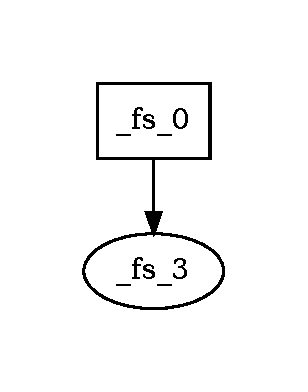
\includegraphics{Diagrams/example4-analysis.pdf}}
\caption{Results of leak analysis on \ttt{example4}}
\label{fig:Analysis4}
\end{figure}

A more complicated example is \ttt{example6} in the following:

\begin{lstlisting}[language=Haskell]
example5 :: Cmd ()
example5 = do
  secretArray <- allocSecret @Int 8
  publicArray <- allocPublic @Int 8
  for (0 :: Expr Public Int) (\i -> ((i <? 8), (i += 1), do
    leak <- decl (0 :: Int)
    for (0 :: Expr Secret Int) (\j -> ((j <? (secretArray ! i))
                                      ,(j += 1), do
      leak += 1))
    (publicArray ! i) .= leak))
  secretArrayA <- allocSecret @Int 8
  secretArrayB <- allocSecret @Int 8
  publicArray2 <- allocPublic @Int 8
  secretArrayA .= secretArray
  secretArrayB .= secretArrayA
  for (0 :: Expr Public Int) (\i -> ((i <? 8), (i += 1), do
    leak2 <- decl (0 :: Int)
    for (0 :: Expr Secret Int) (\j -> ((j <? (secretArrayB ! i))
                                      ,(j += 1), do
      leak2 += 1)
    (publicArray2 ! i) .= leak2))
\end{lstlisting}

In the generated code for \ttt{example5}, we have the correspondence between variables in the EDSL code and the
generated C code given in the table in TABLE \ref{table:Names5}. As both the C code generator and the
static analysis tool use the same name generator, these names stay stable across the results of both. The analysis of \ttt{example5} is given in Fig. \ref{fig:Analysis5}.

\begin{table}[h]
  \centering
  \begin{tabular}{|c|c|}
    \hline
    EDSL name & Generated C Name \\
    \hline
    \verb|secretArray| & \verb|_fs_0|\\
    \verb|publicArray| & \verb|_fs_1|\\
    \verb|leak| & \verb|_fs_3|\\
    \verb|secretArrayA| & \verb|_fs_5|\\
    \verb|secretArrayB| & \verb|_fs_6|\\
    \verb|publicArray2| & \verb|_fs_7|\\
    \verb|leak2| & \verb|_fs_9|\\
    \hline
  \end{tabular}
\caption{Correspondence between EDSL names and generated C names for \ttt{example5}}
\label{table:Names5}
\end{table}

\begin{figure}[h]
\centering
  \resizebox{0.3\columnwidth}{4cm}{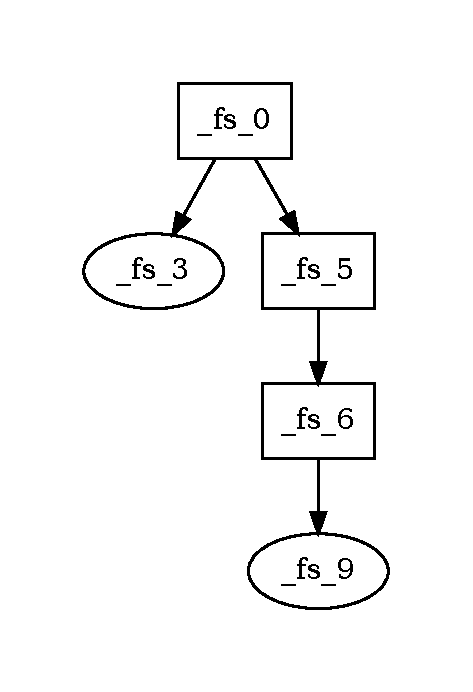
\includegraphics{Diagrams/example5-analysis.pdf}}
\caption{Results of leak analysis on \ttt{example5}}
\label{fig:Analysis5}
\end{figure}


\begin{figure}[h]
  \centering
\resizebox{0.68\linewidth}{!}{
\begin{minipage}{\linewidth}
  \centering
\begin{gather*}
  \inference{%
    \Delta;\Gamma \vdash \ttt{x :: $\tau$}
    \\ \Delta;\Gamma \vdash \ttt{k :: Expr Public $\tau$ $\rarr$ Cmd $\alpha$}
    \\ \Delta;\Gamma\vdash A(\ttt{decl v >>= ($\lambda$x $\rarr$ k)})
    }
    {%
      \Delta,Pub(x);\Gamma \vdash A(\ttt{k})
    }\\
    \\
  \inference{%
    \Delta;\Gamma \vdash \ttt{x :: Expr Public $\tau$}
    & \Delta;\Gamma \vdash \ttt{y :: Expr Public $\tau$}
    \\ \Delta;\Gamma \vdash \ttt{k :: () $\rarr$ Cmd $\alpha$}
    & \Delta;\Gamma \vdash A(\ttt{(x .= y) >>= k})
    \\ \Delta;\Gamma \vdash L(\ttt{x}) \neq \varnothing
    }
    {%
      \Delta;\Gamma \vdash \ttt{x} \sarr L(\ttt{x})
    }\\
  \\
  \inference{%
    \Delta;\Gamma \vdash \ttt{cond :: Expr Bool}
    & \Delta;\Gamma \vdash \ttt{body :: Cmd $\alpha$}
    \\ \Delta;\Gamma \vdash A(\ttt{while cond body})
    & \Delta;\Gamma \vdash s \in Secrets(\ttt{cond})
    \\ \Delta;\Gamma \vdash Pub(\ttt{x})
    }
    {%
      \Delta, s \in L(\ttt{x});\Gamma \vdash A(\ttt{body})
    }\\
  \\
  \inference{%
    \Delta;\Gamma \vdash \ttt{cond :: Expr Bool}
    \\ \Delta;\Gamma \vdash \ttt{t :: Cmd $\alpha$}
    & \Delta;\Gamma \vdash \ttt{f :: Cmd $\alpha$}
    \\ \Delta;\Gamma \vdash A(\ttt{if cond t f})
    & \Delta;\Gamma \vdash s \in Secrets(\ttt{cond})
    \\ \Delta;\Gamma \vdash Pub(\ttt{x})
    }
    {%
      \Delta, s \in L(\ttt{x});\Gamma \vdash A(\ttt{t})
    }\\
  \\
  \inference{%
    \Delta;\Gamma \vdash \ttt{cond :: Expr Bool}
    \\ \Delta;\Gamma \vdash \ttt{t :: Cmd $\alpha$}
    & \Delta;\Gamma \vdash \ttt{f :: Cmd $\alpha$}
    \\ \Delta;\Gamma \vdash A(\ttt{if cond t f})
    & \Delta;\Gamma \vdash s \in Secrets(\ttt{cond})
    \\ \Delta;\Gamma \vdash Pub(\ttt{x})
    }
    {%
      \Delta, s \in L(\ttt{x});\Gamma \vdash A(\ttt{f})
    }\\
  \\
  \inference{%
    \Delta;\Gamma \vdash v \in L(\ttt{x})
    }
    {%
      \Delta;\Gamma \vdash L(\ttt{x}) \neq \varnothing
    }
\end{gather*}
\end{minipage}}
  \caption{Information flow analysis rules which define the relation $\sarr$}
\label{fig:FlowRules}
\end{figure}
...

% \section{Your System}
% ...
% \section{Evaluation}
% ...

\section{Future Work}
A further investigation into the tradeoffs and possible additional features of
the information flow analysis is likely to be useful. This could provide a more
accurate and succinct picture to programmers of where leaks are occurring, or
potentially occurring. It is possible that some of these other leak conditions
could be incorporated into the type system, by exploiting the dependent type
features enabled by singletons~\cite{SingletonsPaper} and, in the future, by Dependent Haskell.~\cite{DepHaskSpec}
Dependent types provide a powerful technique for writing programs at a type-level, which
will be executed at compile-time by the type checker.~\cite{CertProg}

Additionally, features to safely convert between sensitivity levels could prove
useful. A conversion from public to secret would be straightforward. A situational conversion
going the other direction could be provided by an instruction in the EDSL
which might perform a Spectre mitigation measure, such as a cache flush. \cite{PLtea-james}

\section{Conclusion}
...
%-------------------------------------------------------------------------

\bibliographystyle{plain}
\bibliography{reference}
\end{document}
